\chapter{Lezione 2}
\section{La cinematica}
La cinematica è una parte della fisica che si occupa di descrivere il moto. In particolare, utilizzeremo l'algebra dei vettori vista nella lezione precedente e cercheremo, appunto, di descrivere il moto.

Durante il corso, ci limiteremo a studiare il caso in cui l'oggetto che si muove è un \textbf{corpo puntiforme}; questo vuol dire che le dimensioni di tale oggetto sono trascurabili, rispetto al moto che compie. Un'altra considerazione da fare è che faremo una trattazione, che vale nelle misure in cui le velocità che caratterizzano i moti che studieremo, sono molto più piccole della velocità della luce.

\subsection{Definizione di moto}
Il moto è un concetto relativo (nel senso che un corpo è in moto rispetto a un altro); \textbf{un corpo è in un moto relativo rispetto a un altro, quando cambia nel tempo la sua posizione rispetto all'altro corpo}. La condizione opposta al moto si chiama \textbf{quiete}. 

\subsection{Sistema di riferimento}
Prima di descrivere in termini matematici che cos'è il moto, dobbiamo introdurre il concetto di sistema di riferimento.

Possiamo pensare ad un sistema di riferimento, come un'insieme di oggetti che sono in quiete uno rispetto all'altro (la loro posizione relativa non cambia), che sono in quiete rispetto all'osservatore che vuole descrivere il moto. 
\newpage
Questi oggetti sono generalmente rappresentati da una terna di assi cartesiani.

\begin{figure}[h]
\begin{center}
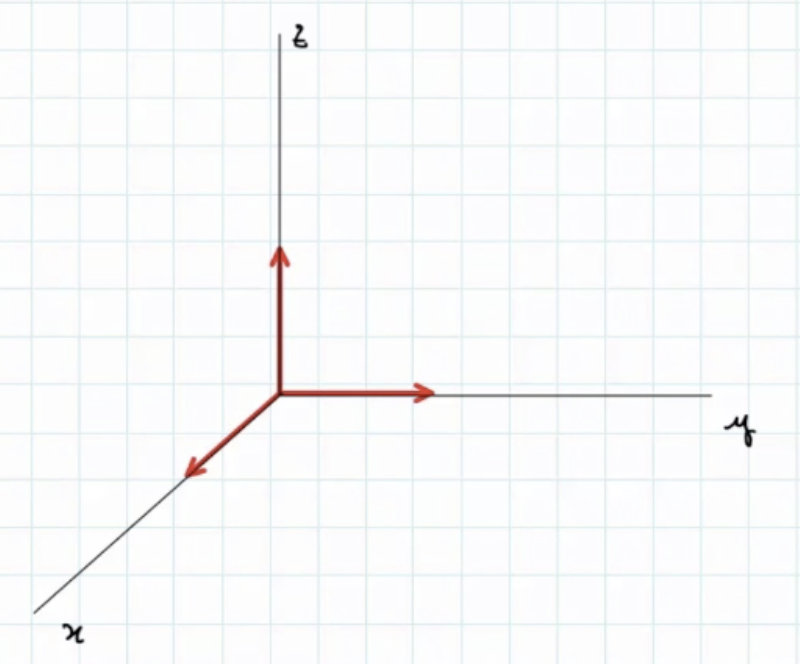
\includegraphics[width = 0.5 \textwidth]{lezione2/images/sistema riferimento1.png}
\label{fig:riferimento1}
\caption{Rappresentazione grafica di un sistema di riferimento}
\end{center}
\end{figure}

Possiamo scrivere gli assi cartesiani, come se fossero tre versori: In particolare, indichiamo l'asse delle $ x $ con il versore $ \overrightarrow{i} $ , le $ y $ con il versore $ \overrightarrow{j} $ e l'asse $ z $ con il versore $ \overrightarrow{k} $ .
L'origine del sistema di riferimento viene indicata con $ O $

\begin{figure}[h]
\begin{center}
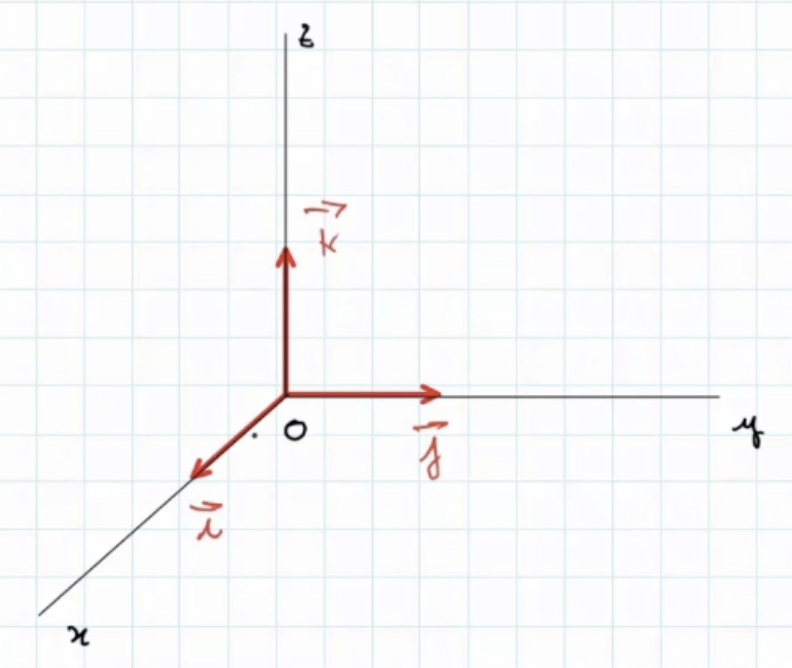
\includegraphics[width = 0.5 \textwidth]{lezione2/images/sistema riferimento2}
\label{fig:riferimento2}
\end{center}
\end{figure}

Se prendiamo come sistema di riferimento quello rappresentato in figura, abbiamo che la posizione di un oggetto a un certo istante $ t $ , è determinata da un \textbf{vettore posizione} definito con le componenti cartesiane. 
\newpage
Questo vettore posizione, rappresenta (in questo caso), la posizione iniziale dell'oggetto di cui stiamo descrivendo il moto. 

\begin{figure}[h]
\begin{center}
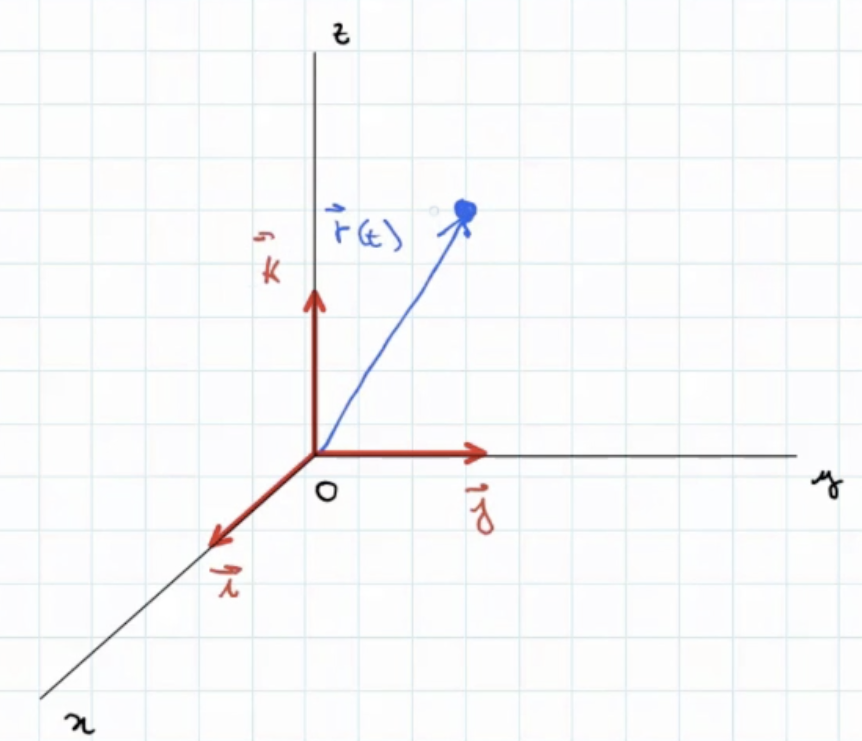
\includegraphics[width = 0.5 \textwidth]{lezione2/images/sistema riferimento3}
\label{fig:riferimento3}
\end{center}
\end{figure}

Abbiamo detto che un oggetto è in moto se la sua posizione (dove per posizione si intende proprio il vettore posizione) cambia nel tempo. Ciò vuol dire che: se chiamiamo $ t + \Delta t $ un certo intervallo di tempo trascorso dall'istante iniziale $ t $ , il vettore posizione sarà differente.

\begin{figure}[h]
\begin{center}
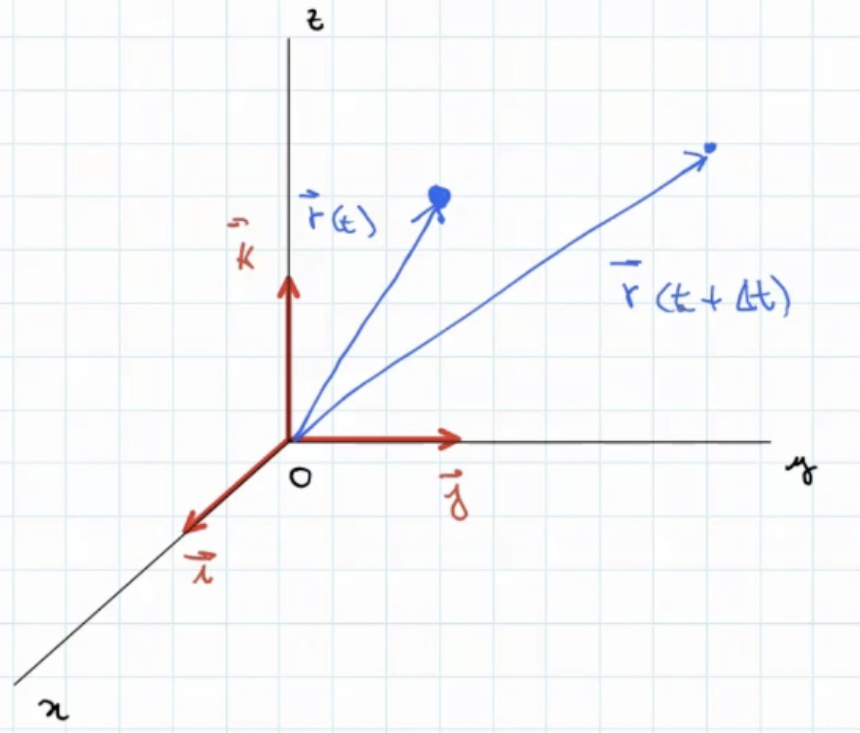
\includegraphics[width = 0.5 \textwidth]{lezione2/images/sistema riferimento4}
\label{fig:riferimento4}
\end{center}
\end{figure}

Per indicare di quanto è variato il vettore posizione, si introduce il \textbf{vettore spostamento}, che non è nient'altro che la differenza di questi due vettori posizione. Se chiamiamo $ \Delta \overrightarrow{r} $ il vettore spostamento
$$ \Delta \overrightarrow{r} = \overrightarrow{r} ( t + \Delta t) - \overrightarrow{r} ( t ) $$

Per rappresentare graficamente questo vettore, dobbiamo utilizzare la regola del parallelogramma; prima di procedere, però ricordiamoci che questa differenza che rappresenta il vettore spostamento, può essere riscritta come
$$ \Delta \overrightarrow{r} = \overrightarrow{r} ( t + \Delta t) + ( - \overrightarrow{r} ( t ) ) $$
\newpage
In pratica stiamo utilizzando il vettore opposto a $ \overrightarrow{r} (t) $

\begin{figure}[h]
\begin{center}
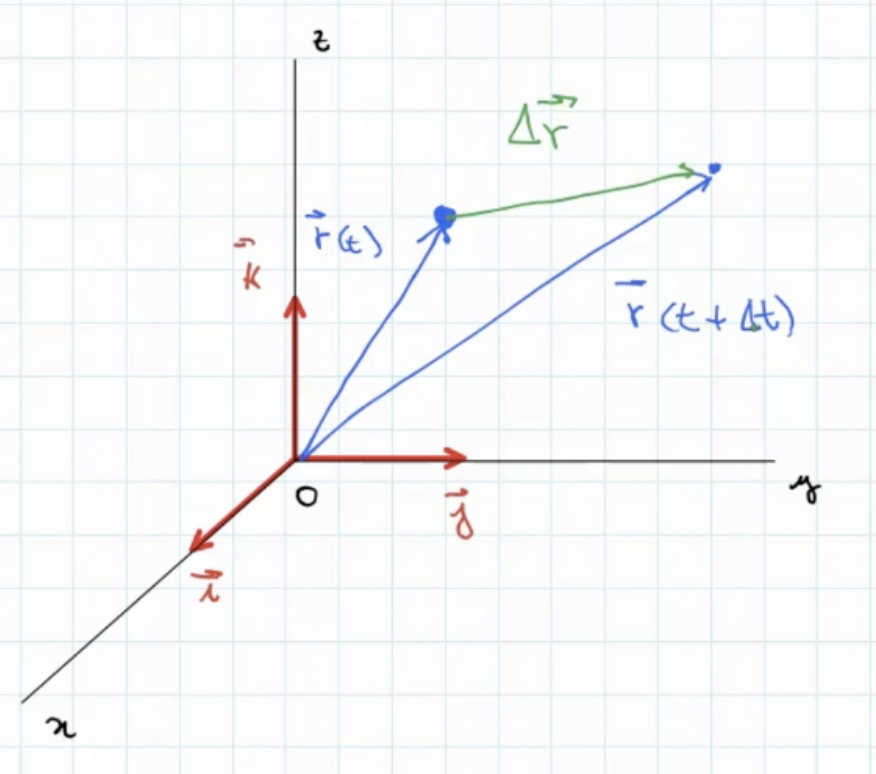
\includegraphics[width = 0.5 \textwidth]{lezione2/images/sistema riferimento5}
\label{fig:riferimento5}
\end{center}
\end{figure}

Si può verificare che se facciamo la somma  $ \delta \overrightarrow{r} + \overrightarrow{r} ( t ) $ effettivamente otteniamo il vettore $ \overrightarrow{r} ( t + \delta t ) $ , cioè il vettore posizione all'istante $ t + \Delta t $ .

Per descrivere il moto dobbiamo introdurre due quantità: la \textit{velocità} e l'\textit{accellerazione}.

Definiamo come \textit{Velocità Media} il rapporto tra il vettore spostamento e il tempo che è intercorso 
tra l'istante $ t + \Delta t$. 


$Velocità\   media \overrightarrow{v}_{media} =\frac{\Delta \overrightarrow{r} }{\Delta t} $ 


Per come è definita, abbiamo la differenza di due vettori $\Delta \overrightarrow{r} $
moltiplicata per $\frac{1}{\Delta t}$ che è uno scalare, quindi il risultato è sempre
un vettore. 
Le unità di misura della velocità media sono quelle del modulo dello spostamento
diviso quelle del tempo, dimensionalmente quindi $[V_{media}= \frac{L}{T} ]$ dove $[\Delta\overrightarrow{r}]= L$
$[\Delta t]= T$ (Le prantesi quadre indicano che ci riferiamo alle unità di misura e non al valore).

La velocità media ovviamente non ci "soddisfa" a pieno perchè qualunque spostamento
originato e termianto nello stesso punto, qualunque fosse il percorso, avrebbe
la stessa velocità media a parità del tempo impiegato.

Introduciamo la \textit{velocità istantanea} 
\begin{equation} 
    \overrightarrow{V}_{istantanea}= 
    \lim_{\Delta t \to 0} \overrightarrow{V}_{media} = 
    \lim_{\Delta t \to 0} \frac { \overrightarrow{r}(t+\Delta t) * \overrightarrow{r}(t) }{\Delta t} = 
    \diffp{\overrightarrow{r}}{t}
\end{equation}

Anche la velocità istantanea come quella media è un vettore e dato che
abbiamo $\frac {t +\Delta t} {t}$ dove $\lim_{\Delta t \to 0}$  è un limite che tende a $0$,
può essere pensata come una derivata.
Ovviamente  le dimensioni di \textit{velocità media}
saranno sempre $[V]=\frac{L}{T}$.
 Essendo un vettore possiamop esprimere la velocità media
 secondo le sue componenti cartesiane 
 $\overrightarrow{v}= v_{x}\overrightarrow{i} + v_{y}\overrightarrow{j} + v_{z}\overrightarrow{k}$

Le componenti sono legate alla velocità in questo modo:
$v^2= \overrightarrow{v}*\overrightarrow{v}= v_{x}^2+v_{y}^2+v_{z}^2$

Per descrivere la posizione del corpo puntiforme, come
così come abbiamo introdotto prima la velocità media e poi la
velocità istantantanea, analogamente anche il vettore velocità istantantanea
cambia nel tempo. Abbiamo bisogno di qualcosa che ci dica \textit{di quanto}
cambia la velocità istantanea. 


Se in un istante $t$ ha velocità $\overrightarrow{v}(t)$, 
dopo un certo tempo avrà  $\overrightarrow{v}(t +\Delta t)$ e quindi 
possiamo introdurre l'\textit{accellerazione media}
\begin{equation}
    \overrightarrow{a}=
    \frac{\overrightarrow{v}(t +\Delta t) - \overrightarrow{v}(t)}{\Delta t} 
\end{equation}

Le unità di misura sono
 $[A_{media}]=\frac{[v]}{[\Delta t]}= \frac{L/T}{T}=\frac{L}{T^2}$

A

